\documentclass{iitsrc}
\usepackage{graphicx}
\usepackage{mflogo}
\usepackage[utf8]{inputenc}%some compilers use utf8x and need the prerendredUnicode characters
%\PrerenderUnicode{áäčďéíľĺňóôŕšťúýžÁÄČĎÉÍĽĹŇÓÔŔŠŤÚÝŽ}
\usepackage{amsmath}
\usepackage{algorithm}
\usepackage[noend]{algpseudocode}

% Please do not remove the following commands:
\editpages{1}{8}

\title{Interactive System for Creation of Notes}
\titlerunning{Interactive System for Creation of Notes}
\author{Martin}{Nemček}
\supervision{\bc}
            {\info}
            {Miroslav Blšták}
            {\iise, \fiit}
\mail{xnemcekm@stuba.sk}
\field{To Be Added by Editor}

\begin{document}

\begin{abstract}
	We are overwhelmed by information from various topics. The challenge in education is to create notes which covers important subset of information. There are known methods to extract information from text. In this article we propose a system to extract the notes from text which are important for educational purpose, so it should create personalized notes for students. We use mainly syntactic text analysis. Notes are created by help of part-of-speech tags and dependencies between words in sentences. The outcome will be an interactive system for creating notes based on learned rules from user.
\end{abstract}

\section{Introduction} \label{introduction}
	Nowadays, we are overwhelmed with huge amount of data and information. %Many of those are duplicates or with slight modification. While searching for a relevant information, we have to get through all of that irrelevant data. Lot of information is in form of texts on internet or in book. The problem is to select useful subset of information from text or text corpuses while not spending too much time on it.
	
	%Substantial group of people who are searching for information and trying to choose the most relevant parts are students. If students spend too much time by extracting relevant information from texts, they tend to loose motivation or feel depressed and they surely could do something more useful. We focus on education and try to create system which would be able to help students with creating notes from texts. 
	
	Computers are not able to understand information in natural language. In our proposed system the notes are created from sentences by extracting relevant information from them. We use syntactic analysis of sentences and extract relations and dependencies between words from these sentences. The final result of our proposed method are personalized notes. The user will be able to modify the automatically created notes. The system will then learn new rules for sentence to note transformation from these changes and takes them into account for the next time.
	
\section{Summarization in natural language processing}	\label{sec:summarization_nlp}
	Note creation is a type of text summarization which attempts to extract the most important and the most relevant information from text. However, it is more personalized and user-specific task than ordinary text summarization. In case of note creation there are the text transformation rules created by user. These rules are used to create notes that best fit particular user's needs. 
	%However beside that it tries to be more personalized and user specific by learning how user creates notes from changes which user can make to created notes by our proposed system. \\

	Author in~\cite{Radev2002} defines a result of summarization as ``A text that is produced from one or more texts, that conveys important information in the original text(s), and that is no longer than half of the original text(s) and usually	significantly less than that.''. Automatic summarization has three important aspects~\cite{Das07asurvey}:
	\begin{itemize}
		\item Summaries may be produced from a single document / text or multiple documents / texts,
		\item Summaries should preserve important information,
		\item Summaries should be short.
	\end{itemize}

	Summarization systems take one or more texts as input and produce concise summary of the most important information in input. Finding the most important information presupposes the ability to understand the semantics of text. Writing a concise summary~\cite{NenkovaMcKeownAutomaticSummarization} requires the capability to reorganize, modify and merge information expressed in different sentences from input.
	
	%Summarization methods can be classified into two groups: \textit{Extractive} and \textit{Abstractive summarization}. An Extractive summarization defined by author in~\cite{GuptaSummarization} is ``summarization method consists of selecting important sentences, paragraphs etc. from the original document and concatenating them into shorter form. The importance of sentences is decided based on statistical and linguistic features of sentences.'' An Abstractive summarization~\cite{GuptaSummarization} is a method that consists of understanding the original text and re-telling it in fewer words. It uses linguistic methods to examine and interpret the text and then to find the new concepts and expressions to best describe it by generating a new shorter text that conveys the most important information from the original text document.

\section{Our proposed system}
	\subsection{Usage of dependencies in note creation} \label{sub:dependencies_in_note_creation}
		At Stanford University a tool named \textit{StanfordNLP}\footnote{www.nlp.stanford.edu} is being developed. The tool is composed of several software such as \textit{Stanford Parser}, \textit{Stanford POS Tagger}, \textit{Stanford EnglishTokenizer} and \textit{Stanford Relation Extractor}. These software focus on tasks of natural language processing. They are implemented primarily in Java, but are also available in other programming languages such as C\#, PHP or Python.
	
		One of the most popular tools for natural language processing is StanfordNLP\footnote{www.nlp.stanford.edu}. It allows to extract dependencies. \textit{Identification of dependencies} gives us simple description of grammatical relations between words in sentence. The dependency consist primarily from two tokens (words) - a governor token and a dependent token and also include the type of relation between those tokens.
		By applying dependency identification on sentence ``Bell, based in Los Angeles, makes and distributes electronic, computer and building products.'' a dependency tree (see Figure~\ref{fig:dependency_tree}) is created~\cite{StanfordDepManual}.
	
		\begin{figure}[h]
			\begin{center}
				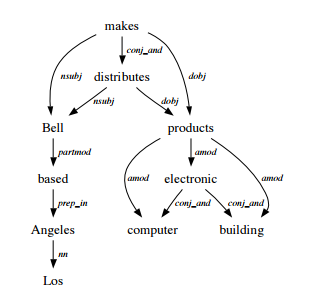
\includegraphics[scale=0.5]{dependency_tree}
				\caption{Dependency tree~\cite{StanfordDepManual}}
				\label{fig:dependency_tree}
			\end{center}
		\end{figure}
	
		In oriented graph like the one in Figure~\ref{fig:dependency_tree} words represent nodes and edges are represented by relations between words.
	
		In our example on Figure~\ref{fig:dependencies_in_sentence} there are relations between words in pairs. Between words \textit{She} and \textit{looks} is relation with name \textit{nominal subject} (nsubj), between \textit{looks} and \textit{beautiful} is adjectival complement (acomp) and between words \textit{very} and \textit{beautiful} is relation called adverb modifier (advmod) ~\cite{StanfordDepManual}.
	
		Dependency beside other thing is composed of governor and dependent token and relation between them. In Figure~\ref{fig:dependencies_in_sentence} is shown that among others there is a dependency which governor token is \textit{looks}, dependent token is \textit{She} and relation is \textit{nsubj}.
	
		\begin{figure}[h]
			\begin{center}
				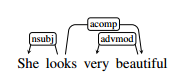
\includegraphics[scale=0.9]{dependencies_in_sentence}
				\caption{Dependencies in sentence~\cite{StanfordDepManual}}
				\label{fig:dependencies_in_sentence}
			\end{center}
		\end{figure}
	
	\subsection{Text processing} \label{sub:data_collection}
		For our experiments we used educational articles from \textit{Wikipedia}\footnote{www.wikipedia.org} written in simple English.	We split these articles into our text database to three collections: texts, sentences and rules. \textit{Text collection} holds whole texts which are processed. \textit{Sentences collection} keeps sentences of texts from text collection. For each sentence in this collections there also is a note which was created by processing the sentence. Last collection named \textit{Rules} holds rules for creating notes from sentences of texts.
	
	\subsection{Rules for processing}	\label{rule}
		A rule consists mainly from two parts - \textit{list of data of original sentence} and \textit{list of data of note}. Each entry in \textit{list of data of original sentence} and \textit{list of data of note} contains these parts: relation name and list of grouped dependencies with the same relation name. Each dependency contains a governor token, a dependent token and its position considering all dependencies. The governor and dependent token consists of Part-Of-Speech (POS) tag and index of word in sentence to which is the token connected. Index of the token is bounded with a position of its word in sentence.
		
		Dependencies from the second list are applied to sentence to create a new note. The rule may order to create a compound note from a sentence. The compound note is composited of some simple sentences. The positions in sentence on which the note should be split into smaller sentences are kept within the rule. \\
		
		When processing a sentence an applicable rule has to be looked up in database before creation of the note. Dependencies of rule and dependencies of the sentence being processed has to correspond to each other. Evaluation is based upon two conditions. The sentence that is being processed has to have the exact amount of entries in list of data of original sentence while these entries contain exactly the same relation names as the rule's relation names.
			
		The applicable rule is found if these two conditions are met. However, the conditions can cause a situation that more than one rule is found. In this case we have to calculate the match probability of this sentence and the original sentence obtained from the rule. The rule with the highest probability of the match is applied.
			
		Calculating the match consists of several steps. First, the POS tags match of governor and dependent tokens is calculated separately. Indices of governor and dependent tokens are calculated also separately. These first steps determine if the sentence contains arbitrary dependency with same value of POS tag or index. In followed step is determined a half-match of dependencies. Half-match of dependency is match of POS tag and index at the same time at governor or dependent token of dependency. We calculate matches of POS tags and index of governor or dependent token for every dependency. Finally, in the last step we calculate the number of absolute-matched dependencies. Absolute-match dependencies is the total match of POS tags and indices in governor and dependent tokens. Every step has assigned a rating. If a condition in the step is evaluated as true, the rating of the step is added to the final result. The final result is a percentage value of the match. The rating is based on importance of the step in calculating a precise match, while depending on the number of steps and dependencies, so the final result cannot exceed a limit of 100\%. A pseudo code for an algorithm calculating the match is outlined in Algorithm~\ref{alg:calculating_match} and specific example is shown on Figure \ref{fig:sentences}.  \\
			
		\begin{algorithm}
			\caption{Calculating match}\label{alg:calculating_match}
			\begin{algorithmic}[1]
				\Procedure{CalculateMatch}{$sentence, originalDependencies$}
				%\State $oneCompareType = \text{100 / count(comparisons)}$
				\State $oneCompareTypeRating \gets \text{calculate percentage rating of one comparison}$
				%oneCompareType \text{ / count(originalDependencies)}$
				
				\ForAll {$originalDependencies$}
					\If {$\text{count(}sentence\text{, }dependency\text{) =  count(}originalDependencies\text{, }dependency\text{)}$}
						\State $match \gets match \text{ + } oneCompareTypeRating$
					\EndIf
					\State $counter \gets counter \text{ + } \text{count(}originalDependencies\text{, } dependency\text{)}$
				\EndFor
				
				\State $oneCompareTypeRating \gets oneCompareType / counter$
				\ForAll {$originalDependency$}
					\ForAll {$dependency$}
						\ForAll {$comparison$}
							\If {$\text{applyComparison(}sentence, comparison, dependency\text{)}$}
								\State $match \gets match \text{ + } oneCompareTypeRating$
							\EndIf
						\EndFor
					\EndFor
				\EndFor
				
				\Return $match$
				\EndProcedure
			\end{algorithmic}
		\end{algorithm}
	
		If rule look up does not find any applicable rule, it means that the system have not processed the same or similar sentence yet. A manual rules of parser are used in this case. The output of the parser is a note. A new rule is created based on the note. Dependencies of original sentences are taken and used to create a \textit{list of data of original sentence}. This list is then assigned to the rule. Dependencies of note are used to create a \textit{list of data of note} which is then also assigned to the rule. The sentence ends are determined depending on how many sentences the note contains. POS tags and indices of tokens are stated by the corresponding words of the original sentence and the newly created note.
		
	\subsection{Rule application}	\label{rule_application}
		By the principle of rule look up, the sentence being processed has to contain dependencies from the \textit{list of data of original sentence} and also dependencies from the \textit{list of data of note}.
	
		The process of applying a rule has several steps. For each dependency in the list of data of original sentence, the respective dependency is looked up in sentence that is being processed. The word corresponding with dependent token from the looked up dependency is taken and added to the note on its index position. In case of dependency relation \textit{nominal subject} the word corresponding with governor is also added. After processing all dependencies the last minor changes are done such as capitalization of the first letter of the note, splitting note into more sentences if rule defined so. Algorithm~\ref{alg:applying_rule} shows pseudo code of the process of applying rule on sentence.
	
		\begin{algorithm}
			\caption{Applying rule}\label{alg:applying_rule}
			\begin{algorithmic}[1]
				\Procedure{ApplyRule}{$sentence, rule$}
				\State $note \gets \text{new Note}$
				\ForAll {$ruleDependencies$}
				\State $dependency \gets \text{findDependency(} sentence \text{, } ruleDependency \text{)}$
				\If {$\text{isFound(}dependency\text{)}$}
				\State $\text{add(} note \text{, getDependent(} dependency \text{))}$
				\If {$\text{isNominalSubject(relation(}dependency \text{))}$}
				\State $\text{add(} note \text{, getGovernor(} dependency \text{))}$
				\EndIf
				\EndIf
				\EndFor
				
				\State $\text{splitToSentences(} note \text{, sentencesEnds(} rule \text{))}$	
				
				\Return $note$
				\EndProcedure
			\end{algorithmic}
		\end{algorithm}
	
	\subsection{Example} \label{subsec:example}
		\begin{figure}[h]
			\begin{center}
				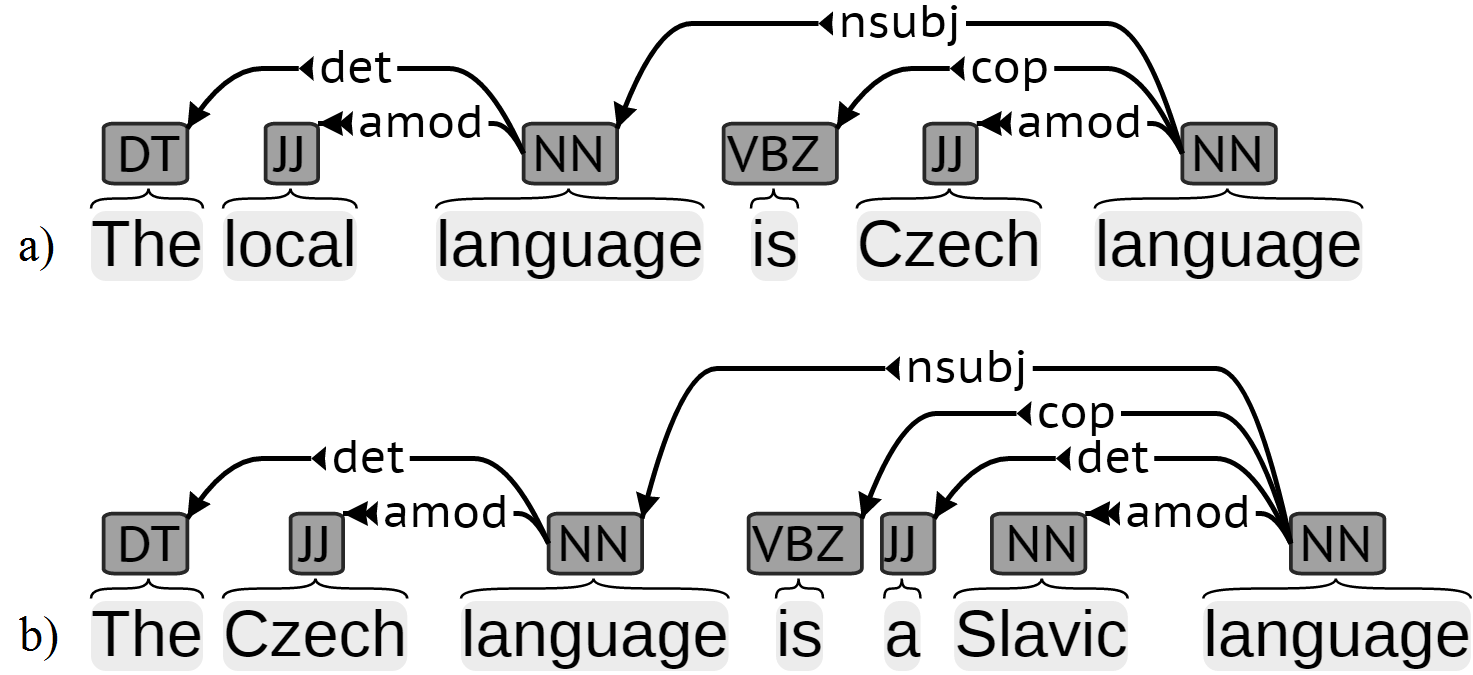
\includegraphics[scale=0.2]{sentences_bw}
				\caption{Example sentences}
				\label{fig:sentences}
			\end{center}
		\end{figure}
		
		Lets consider example from Figure 1. We have rules for two sentences and we are processing the first one. In this situation, there are at least two rules which are applicable for the sentence \textit{a}. Assume that we are calculating match with the sentence \textit{b}. We iterate over all dependencies of processed sentence \textit{a}. The first dependency is \textit{det} with the governor token NN (noun) and index 3 and the dependent token DT (determiner) and index 1. First, we find out, if the sentence \textit{b} contains any dependency with tokens NN or DT and index equals to 1 or 3. This is the separate calculation of POS tags and indices. Then, we try to find in the sentence \textit{b} any dependency, which has dependent or governor token tag of type NN and index equal to 3 or tag of type DT and index equal to 1. This is only the half-match step. As the last step, we check if sentence b contains dependency, where the governor token is NN and index is equal to 3 and the dependent token is DT and its index is 1. If any of these step were matched, the rating of that particular step is added to the final result and iteration continues with following dependency until all dependencies were iterated over.
\section{First experiments}	\label{evaluation}
	We used our system to create notes from three \textit{wikipedia} texts. We compared results with Autosummarizer~\footnote{www.autosummarizer.com}, a project focusing on text summarization. Autosummarizer is still in development and we used a beta version. This system uses an extractive summarization.

	Texts contained 27 sentences and 294 words in total. On Figures~\ref{fig:chart_sentences} and~\ref{fig:chart_words} we show number of sentences and words written to output respectively. Figure~\ref{fig:chart_sentences_not_processed} shows how many sentences from original text were shown in output without being processed. Figure~\ref{fig:chart_words_eliminated} shows average number of irrelevant information (words) that were eliminated from final outputted sentences.
	
	Autosummarization system is better in outputting less amount of data, but it lose lots of relevant information. Our system outputted more data and processed every important information. Our goal is to keep important text information.
%	\begin{figure}
%		\centering
%		\begin{minipage}{.5\textwidth}
%			\centering
%			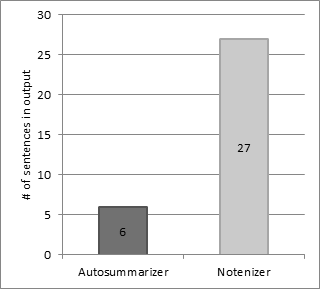
\includegraphics[width=.5\linewidth]{chart_sentences}
%			\captionof{figure}{Number of sentences in output}
%			\label{fig:chart_sentences}
%		\end{minipage}%
%		\begin{minipage}{.5\textwidth}
%			\centering
%			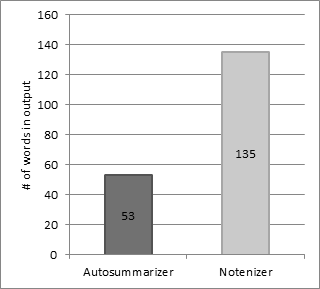
\includegraphics[width=.5\linewidth]{chart_words}
%			\captionof{figure}{Number of words in output}
%			\label{fig:chart_words}
%		\end{minipage}
%	\end{figure}
%		
%	\begin{figure}
%		\centering
%		\begin{minipage}{.5\textwidth}
%			\centering
%			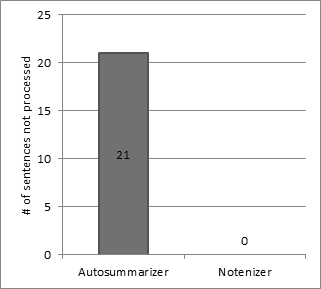
\includegraphics[width=.5\linewidth]{chart_sentences_not_processed}
%			\captionof{figure}{Number of sentences not processed}
%			\label{fig:chart_sentences_not_processed}
%		\end{minipage}%
%		\begin{minipage}{.5\textwidth}
%			\centering
%			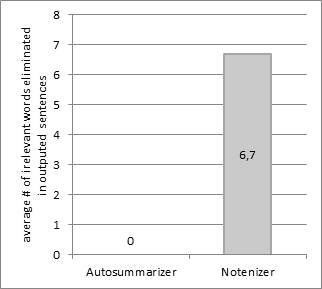
\includegraphics[width=.5\linewidth]{chart_words_eliminated}
%			\captionof{figure}{Number of irelevant words eliminated}
%			\label{fig:chart_words_eliminated}
%		\end{minipage}
%	\end{figure}
%		
%\section{Conclusions and future work}
	When finding a pattern for creating notes from text a lot of possible combinations exists. By combining existing approaches with dependencies and relations the amount of possible combinations is decreased. There is limited number of relations and dependencies and combined with relevant data of texts the number of combinations is lower than if only one approach, for example the part-of-speech tagging is used.
	
	Students are searching for information every day and it is difficult to choose the most relevant parts from text for them. We proposed a system which helps with this. Our system is capable of creating notes from texts. Our system uses \textit{rules} for note creation. A rule is a collection of data such as dependencies, tokens, relations, indices and some other data. The rule is used to extract relevant information from sentence and create a note. Before applying a rule to a sentence, the system looks up applicable rule and calculates match value. We focus to design the system with intent to personalization. User is able to modify the outputted notes and it allows system to learn new patterns and create more personalized notes next time.
	
	The future work can focus on automatization of creation of the notes. By learning rules from interaction with user a general patterns for note creation may be found.
	
\acknowledgement{This work was partially supported by the Scientific Grant Agency of Slovak Republic, grant No. VG 1/0646/15.}

\bibliography{common}
\bibliographystyle{iitsrc}
\end{document}
